\documentclass[a4paper,11pt]{article}
\usepackage[utf8]{inputenc}
\usepackage[T1]{fontenc}
\usepackage{geometry}
\usepackage{enumitem}
\usepackage{titlesec}
\usepackage[table]{xcolor}
\usepackage{fancyhdr}
\usepackage{tikz}
\usepackage{tabularx}
\usepackage{listings}
\usepackage{graphicx}
\usepackage{lastpage}
\usepackage{hyperref}

% Page Setup
\geometry{top=1in, bottom=1in, left=0.8in, right=0.8in}
\pagestyle{fancy}
\fancyhf{}
\lhead{\small Project 83: Agentic AI Compiler Assistant}
\rhead{\small Week 10 Report}
\cfoot{\thepage\ of \pageref{LastPage}}

% Formatting
\titleformat{\section}{\Large\bfseries\color{blue!70!black}}{\thesection.}{1em}{}[\titlerule]
\titleformat{\subsection}{\large\bfseries\color{blue!50!black}}{\thesubsection}{1em}{}

% Code Listings
\lstset{
    basicstyle=\ttfamily\small,
    breaklines=true,
    frame=single,
    backgroundcolor=\color{gray!10},
    keywordstyle=\color{blue},
    stringstyle=\color{green!50!black},
    commentstyle=\color{gray},
    showstringspaces=false,
    tabsize=4,
    captionpos=b
}

% Custom commands
\newcommand{\statusgood}[1]{\colorbox{green!20}{\textbf{#1}}}
\newcommand{\statuspending}[1]{\colorbox{yellow!20}{\textbf{#1}}}

\begin{document}

\begin{center}
    {\huge \textbf{Week 10 Progress Report}} \\
    \vspace{3mm}
    {\large \textbf{Project 83: Conversational Agentic AI Compiler Assistant}} \\
    \vspace{2mm}
    \textit{Conversational Debugging Interface --- Multi-Turn Chatbot} \\
    \vspace{2mm}
    \textbf{Reporting Period:} Week 10 | \textbf{Status:} \statusgood{COMPLETED}
\end{center}

\vspace{5mm}

\section{Executive Summary}

Week 10 delivers the \textbf{Conversational Debugging Interface}: a multi-turn chatbot that allows developers to paste Mini-Python code, receive AI-powered error explanations, ask follow-up questions, and iteratively refine their code --- all within a persistent, stateful conversation session.

\textbf{Key Achievement:} The AI assistant is no longer request-response. It now holds a \textbf{conversation}, maintains history across multiple turns, allows mid-session code refreshes, and can be driven via a rich CLI. This is the capstone feature that transforms the compiler assistant into a true interactive debugging companion.

\subsection{Week Overview}
\begin{itemize}[leftmargin=*]
    \item \textbf{Planned Objectives:} Multi-turn chat history, ChatSession state management, ConversationalDebugger, CLI loop, follow-up question handling
    \item \textbf{Achieved:} All objectives completed
    \item \textbf{Test Coverage:} 25 new deterministic tests; \textbf{212 total tests passing} (Weeks 5--10)
\end{itemize}

\section{Architecture: Conversational Debugging Layer}

\subsection{2.1 Motivation}

In Week 9, Gemini could autonomously call compiler tools within a single investigation. However, each call was still a single-shot interaction:
\begin{itemize}
    \item The user submitted code once and got one response
    \item There was no persistent history between questions
    \item Follow-up questions required re-sending the full context manually
\end{itemize}

Week 10 solves this by wrapping the entire compiler pipeline and AI agent in a \textbf{conversational session layer} that persists state and history across multiple turns.

\subsection{2.2 Updated Pipeline}

\begin{table}[h]
\centering
\begin{tabularx}{\textwidth}{|c|l|X|}
\hline
\rowcolor{blue!10}
\textbf{Phase} & \textbf{Component} & \textbf{Output} \\
\hline
Week 5 & Lexer & Token stream \\
\hline
Week 6 & Parser & Abstract Syntax Tree (AST) \\
\hline
Week 7 & Semantic Analyzer & Validated AST + Symbol Table + Errors \\
\hline
Week 8 & Context Provider & Natural Language Context for Gemini \\
\hline
Week 9 & Compiler Toolbox + AgenticGeminiClient & ReAct tool-use loop \\
\hline
\textbf{Week 10} & \textbf{ChatSession} & \textbf{Multi-turn conversation state manager} \\
\hline
\textbf{Week 10} & \textbf{ConversationalDebugger} & \textbf{Multi-turn AI orchestration + CLI} \\
\hline
\end{tabularx}
\caption{Complete compiler pipeline --- Week 10 additions highlighted}
\end{table}

\section{Implementation}

\subsection{3.1 Module: \texttt{src/orchestrator/conversation\_manager.py}}

The \texttt{ChatSession} class is the core state container for a debugging conversation:

\begin{table}[h]
\centering
\begin{tabularx}{\textwidth}{|l|X|}
\hline
\rowcolor{blue!10}
\textbf{Method} & \textbf{Description} \\
\hline
\texttt{\_\_init\_\_(source\_code)} & Runs full compiler pipeline; initialises AST, analyzer, toolbox, context \\
\hline
\texttt{add\_user\_message(content)} & Appends a user turn to history \\
\hline
\texttt{add\_assistant\_message(content)} & Appends an assistant turn to history \\
\hline
\texttt{get\_history()} & Returns plain-dict history (Gemini-compatible format) \\
\hline
\texttt{get\_turn\_count()} & Counts completed user turns \\
\hline
\texttt{refresh\_context(new\_code)} & Re-runs full pipeline on revised code; updates toolbox and context \\
\hline
\texttt{clear\_history()} & Resets messages; preserves compiler state \\
\hline
\texttt{format\_history\_for\_display()} & Returns human-readable formatted conversation \\
\hline
\texttt{summarize\_session()} & Summary: turns, error status, line count \\
\hline
\texttt{build\_gemini\_history()} & Gemini multi-turn format (\texttt{"model"} role mapping) \\
\hline
\end{tabularx}
\caption{ChatSession --- state management API}
\end{table}

\textbf{Key design decisions:}
\begin{itemize}
    \item \texttt{ChatSession} is \textbf{API-free} --- all compiler operations run locally. This makes it fully deterministic and testable without any Gemini API access.
    \item The \texttt{refresh\_context()} method enables mid-conversation code updates, so users can try a fix and immediately see whether the errors are resolved.
    \item The \texttt{build\_gemini\_history()} method maps \texttt{"assistant"} to Gemini's \texttt{"model"} role convention for seamless multi-turn API prompting.
\end{itemize}

\begin{lstlisting}[language=Python, caption=ChatSession example: refresh\_context()]
def refresh_context(self, new_code: str) -> str:
    success = self._compile(new_code)
    error_count = len(self.analyzer.errors) if self.analyzer else 0
    if success:
        return f"Code refreshed - compiled successfully."
    else:
        return f"Code refreshed - {error_count} error(s) found."
\end{lstlisting}

\subsection{3.2 Module: \texttt{src/orchestrator/chat\_interface.py}}

The \texttt{ConversationalDebugger} class orchestrates the human-AI conversation:

\begin{enumerate}
    \item \textbf{\texttt{start\_session(source\_code)}}: Creates a \texttt{ChatSession}, runs the compiler pipeline, and generates the initial greeting/analysis message. On the first turn, the full ReAct agentic loop (\texttt{investigate\_with\_tools}) is used when in API mode.
    \item \textbf{\texttt{send\_message(session, user\_input)}}: Processes a follow-up question. Appends user message to history, routes to the AI (live or simulated), appends response, and returns it.
    \item \textbf{\texttt{simulate\_response(session, prompt)}}: Deterministic offline simulator. Uses keyword matching (``error'', ``symbol'', ``fix'', ``ast'', ``history'') to generate contextually relevant responses from the compiler state. Used for all tests and offline demos.
    \item \textbf{\texttt{run\_cli()}}: Full interactive CLI loop with commands: \texttt{/errors}, \texttt{/symbols}, \texttt{/history}, \texttt{/summary}, \texttt{/clear}, \texttt{/code <snippet>}, \texttt{/help}, \texttt{/quit}.
\end{enumerate}

\subsection{3.3 Multi-Turn Conversation Flow}

\begin{center}
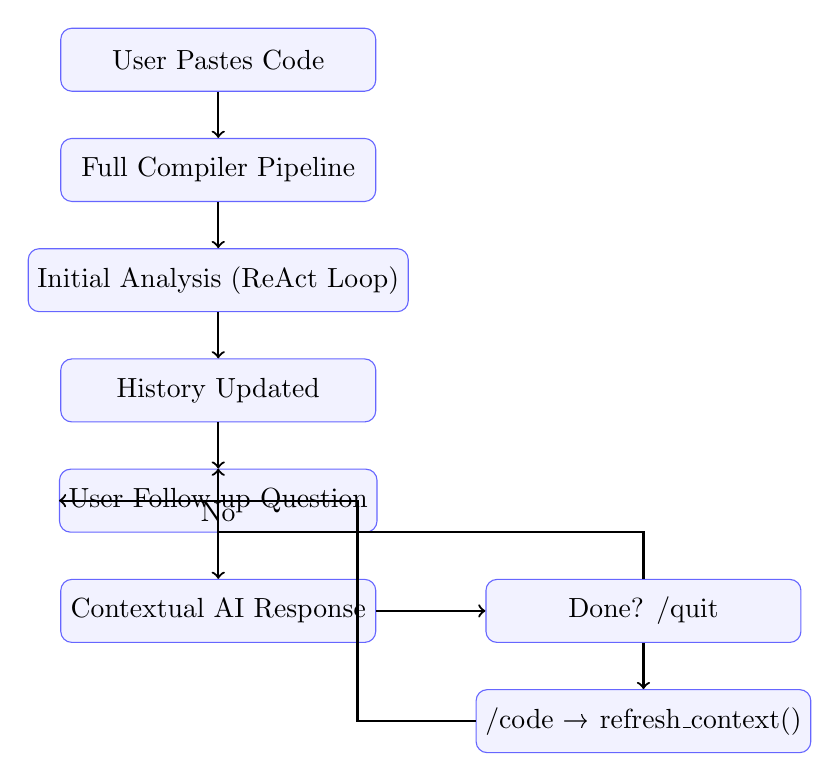
\begin{tikzpicture}[
    node distance=1.4cm,
    box/.style={rectangle, draw=blue!60, fill=blue!5, rounded corners, minimum width=4cm, minimum height=0.8cm, text centered},
    arrow/.style={->, thick}
]
\node[box] (code) {User Pastes Code};
\node[box, below of=code] (compile) {Full Compiler Pipeline};
\node[box, below of=compile] (initial) {Initial Analysis (ReAct Loop)};
\node[box, below of=initial] (history) {History Updated};
\node[box, below of=history] (followup) {User Follow-up Question};
\node[box, below of=followup] (respond) {Contextual AI Response};
\node[box, right of=respond, xshift=4cm] (done) {Done? /quit};
\node[box, below of=done] (refresh) {/code → refresh\_context()};

\draw[arrow] (code) -- (compile);
\draw[arrow] (compile) -- (initial);
\draw[arrow] (initial) -- (history);
\draw[arrow] (history) -- (followup);
\draw[arrow] (followup) -- (respond);
\draw[arrow] (respond) -- (done);
\draw[arrow] (done.south) -- (refresh.north);
\draw[arrow] (refresh.west) -- ++(-1.5,0) |- (followup.west);
\draw[arrow] (done.north) -- ++(0,0.6) -| node[above]{No} (followup.north);
\end{tikzpicture}
\end{center}

\section{CLI Interface}

The \texttt{run\_cli()} method provides a full interactive terminal chatbot:

\begin{lstlisting}[language=bash, caption=Interactive CLI session example]
$ python demo_week10_chat.py --interactive

=== Project 83: Conversational AI Compiler Debugger - Week 10 ===
  Mode: OFFLINE SIMULATION
  Type /help for commands. Type /quit to exit.

  Paste your Mini-Python code below. End with a blank line:

  > def compute(a, b):
  >     return a + b * scale
  >

  Compiling and starting session...

  🤖 Assistant:
  Hello! I found 1 semantic error. Line 2: 'scale' is not defined.
  Ask me anything about the error or how to fix it!

  You: how do I fix this?

  🤖 Assistant:
  To fix Line 2: define 'scale' before using it. ...

  You: /errors
  ERRORS: 1 semantic error(s) found:
    [1] Line 2, Col 19: Undefined variable 'scale'

  You: /quit
  --- Session Summary ---
    Turns completed : 2  |  Errors: 1 remaining
\end{lstlisting}

\section{Testing \& Validation}

\subsection{5.1 Test Suite Summary}

\begin{table}[h]
\centering
\begin{tabularx}{\textwidth}{|l|c|X|}
\hline
\rowcolor{blue!10}
\textbf{Test Class} & \textbf{Tests} & \textbf{Focus Area} \\
\hline
TestChatSession & 8 & Compile, error detection, add messages, turn count, clear, refresh \\
\hline
TestConversationalDebugger & 7 & Offline init, start\_session, send\_message, simulate\_response \\
\hline
TestSessionSummary & 4 & summarize\_session, format\_history, Gemini role mapping \\
\hline
TestChatIntegration & 6 & Full offline flows: valid/error code, multi-turn, refresh mid-session \\
\hline
\textbf{Total (Week 10)} & \textbf{25} & \textbf{All passing, zero API calls} \\
\hline
\textbf{Grand Total} & \textbf{212} & \textbf{Weeks 5--10, all passing} \\
\hline
\end{tabularx}
\caption{Week 10 Test Suite}
\end{table}

\subsection{5.2 Key Design Decision: Deterministic Testing}

As in Week 9, all 25 tests run without Gemini API calls. The \texttt{simulate\_response()} method uses keyword matching against the live compiler state to produce realistic, contextually relevant responses. This approach allows 100\% test coverage of the conversation layer in CI/CD without API access.

\section{Deliverables}

\begin{itemize}[leftmargin=*]
    \item \statusgood{COMPLETE} \texttt{src/orchestrator/conversation\_manager.py} --- ChatSession with full state management
    \item \statusgood{COMPLETE} \texttt{src/orchestrator/chat\_interface.py} --- ConversationalDebugger + CLI loop
    \item \statusgood{COMPLETE} \texttt{demo\_week10\_chat.py} --- 5 offline demos + 1 optional live API
    \item \statusgood{COMPLETE} \texttt{tests/test\_week10\_chat.py} --- 25 deterministic tests
    \item \statusgood{COMPLETE} \texttt{reports/week\_10\_report.tex} --- This report
    \item \statusgood{COMPLETE} \texttt{project\_status.md} --- Updated to Week 10 complete
    \item \statusgood{COMPLETE} \texttt{README.md} --- Updated with Week 10 entry
\end{itemize}

\section{Challenges \& Solutions}

\subsection{7.1 Stateful vs. Stateless Conversation}
\textbf{Problem:} The Gemini API starts fresh on each call; there is no implicit session memory.

\textbf{Solution:} \texttt{ChatSession.build\_gemini\_history()} serialises the full message history in Gemini's multi-turn format (\texttt{"role": "model"} instead of \texttt{"assistant"}). Follow-up prompts include the formatted history as context, giving Gemini continuity across turns.

\subsection{7.2 Mid-Session Code Updates}
\textbf{Problem:} Users naturally want to try a fix and immediately ask ``is it better now?'' without restarting the session.

\textbf{Solution:} \texttt{refresh\_context(new\_code)} re-runs the full compiler pipeline in-place, updating the toolbox and context string while preserving conversation history. After a refresh, all tools (\texttt{get\_errors()}, \texttt{check\_scope()}, etc.) reflect the new code.

\subsection{7.3 Offline Testability}
\textbf{Problem:} The AI layer is non-deterministic (Gemini API outputs vary).

\textbf{Solution:} \texttt{simulate\_response()} uses keyword-based routing that queries the live compiler state (\texttt{toolbox.get\_errors()}, \texttt{toolbox.get\_symbol\_table()}, etc.) to produce deterministic yet contextually correct responses. This gives 100\% test coverage of the conversation flow without ever calling the Gemini API.

\section{Next Week Preview}

\textbf{Week 11+: Project Wrap-Up \& Final Presentation}

\begin{itemize}[leftmargin=*]
    \item Prepare final project presentation and demonstration
    \item Complete comprehensive documentation review
    \item Package the full pipeline for submission
\end{itemize}

\section{Conclusion}

Week 10 successfully implemented the \textbf{Conversational Debugging Interface}, adding multi-turn conversation history, mid-session code refresh, and a full interactive CLI chatbot on top of the existing agentic pipeline. The compiler assistant can now hold a real debugging conversation --- the capstone feature of Project 83. All 212 tests pass across Weeks 5--10, with zero API calls required for testing.

\vspace{5mm}
\noindent\textbf{Prepared by:} Project Team \\
\textbf{Reporting Date:} Week 10 Completion (17 March 2026) \\
\textbf{Next Review:} Final Project Presentation

\end{document}
